%\documentclass[smaller,handout]{beamer}
\documentclass[smaller]{beamer}

\usepackage{amsfonts}
\usepackage{amssymb}
\usepackage{amsmath}
\usepackage{epsfig}
\usepackage{graphicx}
\usepackage{mathtools}
\usepackage{rotating}

\def\F{{\cal F}}
\def\X{{\cal X}}
\def\Y{{\cal Y}}
\def\Z{{\cal Z}}
\def\P{{\mathbb P}}
\def\R{{\mathbb R}}
\def\E{{\mathbb E}}
\def\bZ{{\mathbb Z}}
\def\darkred{\color{red!70!black}}
\def\darkgreen{\color{green!60!black}}
\def\learn{{\mbox{LEARN}}}
\def\err{{\mbox{err}}}
\def\bI{{\tilde{I}}}
\def\dis{{\mbox{DIS}}}

\DeclareMathOperator*{\argmin}{arg\,min}
\DeclareMathOperator*{\argmax}{arg\,max}

%\usepackage{pgfpages}
%\pgfpagesuselayout{4 on 1}[letterpaper,border shrink=5mm,landscape]

%\usepackage{beamerarticle}

\mode<presentation>
{
  \usetheme{default}
%  \setbeamercovered{transparent}
  % or whatever (possibly just delete it)
}


\usepackage[english]{babel}
% or whatever

\useinnertheme{circles}
\usefonttheme{structurebold}

%\usepackage[latin1]{inputenc}
% or whatever

%\usepackage{times}
%\usepackage[T1]{fontenc}
% Or whatever. Note that the encoding and the font should match. If T1
% does not look nice, try deleting the line with the fontenc.

\title{Some linear algebra background}

\author{CSE 250B}
% - Give the names in the same order as the appear in the paper.
% - Use the \inst{?} command only if the authors have different
%   affiliation.

%\institute{University of California, San Diego}

\date{}

% If you wish to uncover everything in a step-wise fashion, uncomment
% the following command: 

%\beamerdefaultoverlayspecification{<+->}
\setbeamertemplate{navigation symbols}{}

\def\vone{{\vskip.1in}}
\def\v2{{\vskip.2in}}
\def\bR{{\mathbb R}}
\def\R{{\mathbb R}}
\def\eps{{\epsilon}}
\def\E{{\mathbb E}}
\def\epso{{\epsilon_o}}
\def\nicered{{\color{red!70!black}}}
\def\pr{{\mbox{\rm Pr}}}

\setbeamercolor{title}{fg=red!80!black,bg=red!20!white}
\setbeamercolor{author}{fg=blue!80!black}

\begin{document}

% *** TITLE ***
\begin{frame}
  \titlepage
\end{frame}

% *** MATRIX-VECTOR NOTATION ***
\begin{frame}
\frametitle{Matrix-vector notation}

{\darkred Vector $x \in \R^p$ and matrix $M \in \R^{r \times p}$:}
$$ x = \begin{pmatrix} x_1 \\ x_2 \\ x_3 \\ \vdots \\ x_p \end{pmatrix},
\ \ 
M = 
\begin{pmatrix} 
M_{11} & M_{12} & \cdots & M_{1p} \\
M_{21} & M_{22} & \cdots & M_{2p} \\
\vdots & \vdots & \ddots & \vdots \\
M_{r1} & M_{r2}  & \cdots & M_{rp}
\end{pmatrix} .$$

\pause\vskip.05in
{\darkred Transpose $x^T$ and $M^T \in \R^{p \times r}$:}
$$ x^T = \begin{pmatrix} x_1 & x_2 & \cdots & x_p \end{pmatrix},
\ \ 
M^T = 
\begin{pmatrix} 
M_{11} & \cdots & M_{r1} \\
M_{12} & \cdots & M_{r2} \\
M_{13} & \cdots & M_{r3} \\
\vdots & \ddots & \vdots \\
M_{1p} & \cdots & M_{rp}
\end{pmatrix} .$$

\pause\vskip.05in
{\darkgreen Properties of transpose: $(A^T)^T = A$ and $(AB)^T = B^T A^T$.}
 
\end{frame}

% *** DOT PRODUCT ***
\begin{frame}
\frametitle{Dot product}

{\darkred Dot product of vectors $x,y \in \R^p$:}
$$ x \cdot y \ = \ x^T y \ = \ x_1y_1 + \cdots + x_py_p .$$

\pause\v2
{\darkgreen This tells us the angle between $x$ and $y$:}

\begin{center}
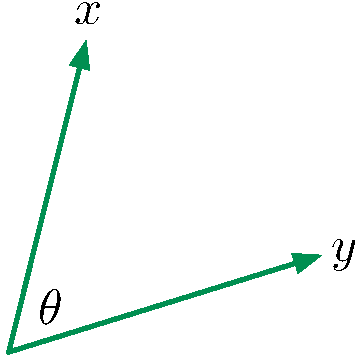
\includegraphics[width=1in]{dotproduct.pdf}
\hskip.25in
\raisebox{.65in}{\begin{minipage}[t]{2in}
$$ \cos \theta \ = \ \frac{x \cdot y}{\|x\|\, \|y\|} .$$ 
\end{minipage}}
\end{center}

\pause
Easiest when $x,y$ are {\it unit vectors} (length 1): then $\cos \theta = x \cdot y$.

\pause\v2
\alert{$x$ is orthogonal (at right angles) to $y$ iff $x \cdot y = $ ??}

\pause\vskip.05in
\alert{What is $x \cdot x$?}

\end{frame}

% *** MATRIX-VECTOR PRODUCT ***
\begin{frame}
\frametitle{Matrix-vector products}

If $M \in \R^{r \times p}$ and $x \in \R^p$ then
$$ Mx \ = \ 
\begin{pmatrix}
\xleftarrow{\hspace*{1cm}} M_1 \xrightarrow{\hspace*{1cm}} \\
\xleftarrow{\hspace*{1cm}} M_2 \xrightarrow{\hspace*{1cm}} \\
\vdots \\
\xleftarrow{\hspace*{1cm}} M_r \xrightarrow{\hspace*{1cm}} \\
\end{pmatrix}
\begin{pmatrix}
\Bigg\uparrow \\
x \\
\Bigg\downarrow
\end{pmatrix}
\ = \ 
\begin{pmatrix}
M_1 \cdot x \\
M_2 \cdot x \\
\vdots \\
M_r \cdot x
\end{pmatrix}
$$

\pause\v2
{\darkred This mapping $x \mapsto Mx$ is a {\bf linear function} from $\R^p$ to $\R^r$:
$$ M(x + x') = Mx + Mx' .$$}

\pause
{\darkgreen If $M \in \R^{p \times p}$ and $x \in \R^p$ then $x \mapsto x^T M x$ is a {\bf quadratic function} from $\R^p$ to $\R$:
$$ x^T M x \ = \ \sum_{i,j = 1}^p M_{ij} x_i x_j .$$}

\end{frame}

% *** QUICK QUIZ ***
\begin{frame}
\frametitle{Quick quiz}

\begin{enumerate}
\item<1-> Write the linear function $f(x_1, x_2) = 3x_1 + 2x_2$ using vector notation (here, $x_1, x_2 \in \R$).
\item<2-> Write the quadratic function $f(x_1, x_2) = x_1^2 + 2x_1x_2 + 3 x_2^2$ using matrices and vectors.
\item<3-> A linear function from $\R^3$ to $\R^3$ is given by the matrix
$$ M \ = \ 
\begin{pmatrix}
1 & 1 & 1 \\
2 & 2 & 2 \\
3 & 3 & 3
\end{pmatrix}
.
$$
As $x$ varies, does $Mx$ fill up all of $\R^3$?

\end{enumerate}

\end{frame}

% *** A HIERARCHY OF SQUARE MATRICES ***
\begin{frame}
\frametitle{A hierarchy of square matrices}

\begin{center}
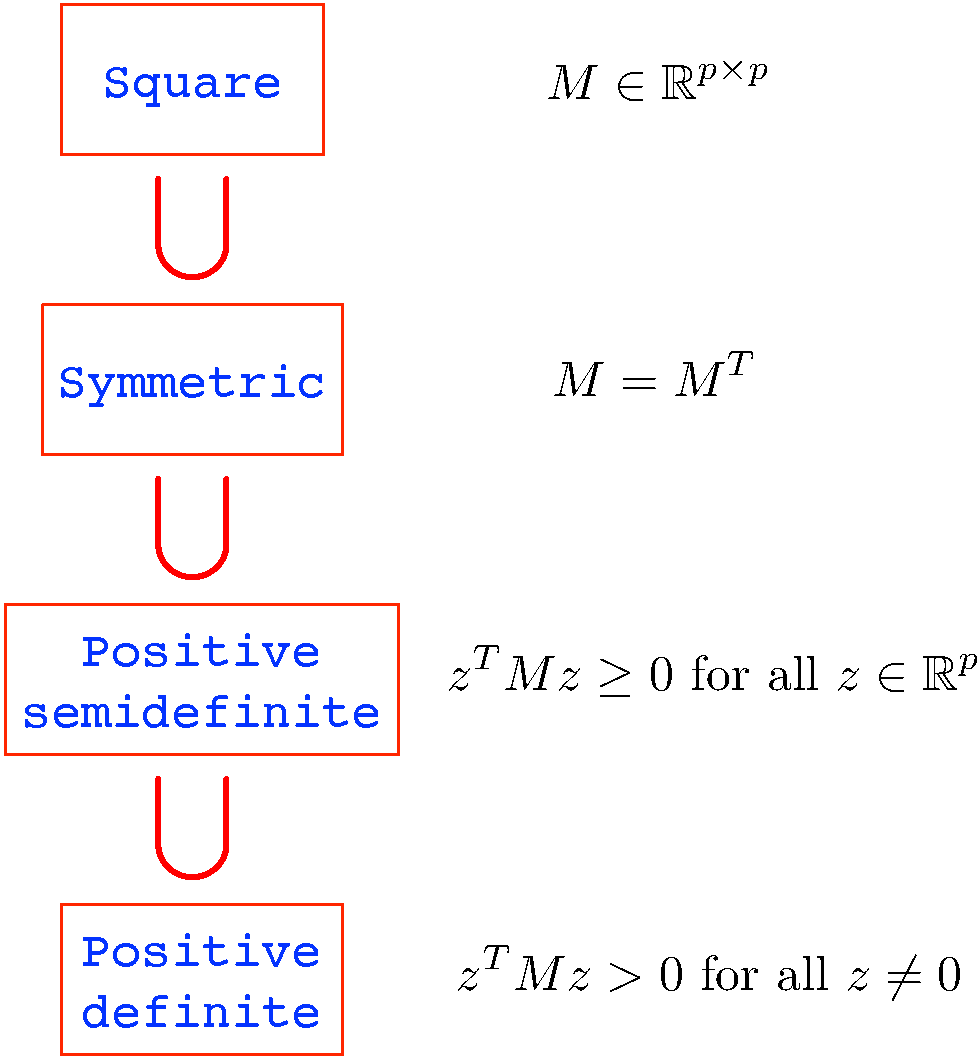
\includegraphics[width=2.5in]{square.pdf}
\end{center}

\end{frame}

% *** QUICK QUIZ ***
\begin{frame}
\frametitle{Quick quiz}

{\darkred Symmetric matrix $M$ is positive semidefinite (psd) if $z^T M z \geq 0$ for all $z$.}

\begin{enumerate}
\item<1-> PSD or not?

\vskip.1in

\begin{itemize}
\item<1-> $\begin{pmatrix} 1 & 1 \\ 1 & 1 \end{pmatrix}$

\vskip.1in

\item<2-> $\begin{pmatrix} 1 & 2 \\ 2 & 1 \end{pmatrix}$
\end{itemize}

\vskip.1in

\item<3-> A diagonal matrix is PSD if and only if ???
\item<4-> Show: If $M, N$ are of the same size and PSD and $M+N$ is PSD.
\end{enumerate}

\end{frame}

% *** Checking if a matrix is PSD ***
\begin{frame}
\frametitle{Checking if a matrix is PSD}

\alert{Useful fact: a matrix $M$ is PSD iff it can be written in the form $UU^T$ for some matrix $U$.}

\pause\v2
Quick check: say $U \in \R^{r \times p}$ and $M = UU^T$.

\begin{enumerate}
\item<3-> $M$ is square.
\item<4-> $M$ is symmetric.
\item<5-> Pick any $z \in \R^r$. Then
\begin{align*}
z^T M z \ = \ z^T U U^T z \ &= \ (z^TU)(U^Tz) \\
&= \  (U^Tz)^T (U^T z) \ = \ \|U^T z\|^2 \ \geq \ 0 .
\end{align*}
\end{enumerate}

\onslide<6->{\darkgreen Another useful fact: any covariance matrix is PSD. (Same argument, along with linearity of expectation.)}

\end{frame}

% *** EIGENVALUES AND EIGENVECTORS ***
\begin{frame}
\frametitle{Eigenvalues and eigenvectors}

\begin{enumerate}
\item<1-> Any matrix $M$ defines a linear transformation $x \mapsto Mx$.
\item<2-> We'd like to understand the nature of these transformations. The easiest case is when $M$ is {\bf diagonal}:
$$
\underbrace{\begin{pmatrix}
2 & 0 & 0 \\
0 & -1 & 0 \\
0 & 0 & 10
\end{pmatrix}}_{M}
\underbrace{\begin{pmatrix} x_1 \\ x_2 \\ x_3 \end{pmatrix}}_{x}
\ \ = \ \ 
\underbrace{\begin{pmatrix} 2x_1 \\ -x_2 \\ 10x_3 \end{pmatrix}}_{Mx}
$$
In this case, $M$ simply scales each coordinate separately.
\item<3-> What about more general matrices that are symmetric but not necessarily diagonal? They also just scale coordinates separately, but in a {\bf different coordinate system}.
\end{enumerate}

\onslide<4->{\darkred 
Let $M$ be a $p \times p$ matrix. 

We say $u \in \R^p$ is an {\bf eigenvector} if $M$ maps $u$ onto the same direction, that is,
$$ Mu = \lambda u$$
for some scaling constant $\lambda$. This $\lambda$ is the {\bf eigenvalue} associated with $u$.}

\end{frame}

% *** EIGENVALUES AND EIGENVECTORS: EXAMPLES ***
\begin{frame}
\frametitle{Eigenvalues and eigenvectors: examples}

{\darkred {\bf
We say $u$ is an eigenvector of $M$, with eigenvalue $\lambda$, if $Mu = \lambda u$.}}

\pause\v2
Question: What are the eigenvectors and eigenvalues of:
$$ M = \begin{pmatrix}
2 & 0 & 0 \\
0 & -1 & 0 \\
0 & 0 & 10
\end{pmatrix} \ ?
$$

\pause
{\darkgreen Answer: Eigenvectors $e_1, e_2, e_3$, with corresponding eigenvalues $2,-1,10$.}

\pause\vskip.05in
Question: Matrix
$M = \begin{pmatrix} 3 & 1 \\ 1 & 3 \end{pmatrix} $ has eigenvectors
$$u_1 = \frac{1}{\sqrt{2}} \begin{pmatrix} 1 \\ 1 \end{pmatrix}, \ \ \ 
u_2 = \frac{1}{\sqrt{2}} \begin{pmatrix} -1 \\ 1 \end{pmatrix} .$$
What are the corresponding eigenvalues?

\pause
{\darkgreen Answer: $\lambda_1 = 4$ and $\lambda_2 = 2$.}

\pause\v2
\alert{In both cases the eigenvectors form an orthonormal basis.}
\end{frame}

% *** EIGENVECTORS OF A REAL SYMMETRIC MATRIX ***
\begin{frame}
\frametitle{Eigenvectors of a real symmetric matrix}

{\bf Theorem.} Let $M$ be any real symmetric $p \times p$ matrix. Then $M$ has
\begin{itemize}
\item $p$ eigenvalues $\lambda_1, \ldots, \lambda_p$
\item corresponding eigenvectors $u_1, \ldots, u_p \in \R^p$ that are {\bf orthonormal}:
$$ u_i \cdot u_j \ = \ 
\left\{
\begin{array}{ll}
0 & \mbox{if $i \neq j$} \\
1 & \mbox{if $i = j$}
\end{array}
\right.
$$

\end{itemize}

\pause\v2
\alert{We can think of $u_1, \ldots, u_p$ as being the axes of the natural coordinate 
system for understanding $M$.}

\pause\v2
{\darkgreen
{\bf Theorem.} Let $M$ be any real symmetric $p \times p$ matrix, and let $\lambda_1, \ldots, \lambda_p$ be its eigenvalues. Then:}
\begin{itemize}
\item {\darkgreen $M$ is positive semidefinite iff every $\lambda_i$ is $\geq 0$.}
\item {\darkgreen $M$ is positive definite iff every $\lambda$ is $> 0$.}
\end{itemize}


\end{frame}

\end{document}
